\documentclass{../latex/utmreport}
\newcommand{\ReportTitle}{Lab 10: Add Your Own System Call: trace}
% Shared title-page and PDF metadata for every laboratory report.
\newcommand{\StudentName}{Gafenco Victor}
\newcommand{\StudentGroup}{FAF-241}
\newcommand{\CourseName}{Operating Systems}
\newcommand{\InstructorName}{Patricia Reițman}
\newcommand{\InstructorTitle}{Assistant lecturer}
\newcommand{\ReportCity}{Chișinău}
\newcommand{\ReportYear}{2026}
\newcommand{\CourseRepository}{https://github.com/yoda-dinmd/os-labs}

\selectlanguage{english}
\utmlogo{../latex/assets/UTM_Logo_English.jpeg}
\institution{Technical University of Moldova}
\faculty{Faculty of Computers, Informatics, and Microelectronics}
\department{Department of Software Engineering}
\studyprogramme{Software Engineering Study Programme}
\documenttype{Laboratory report}
\student{\StudentName}{\StudentGroup}
\supervisor{\InstructorName}{\InstructorTitle}
\renewcommand{\UTMCoordinatorLabel}{Instructor}
\cityyear{\ReportCity}{\ReportYear}
\reportsubtitle{\CourseName}
\hypersetup{pdfauthor={\StudentName},pdfsubject={\CourseName},
  pdftitle={\ReportTitle}}
\reporttitle{\ReportTitle}
\addto\captionsenglish{\renewcommand{\figurename}{Figure}\renewcommand{\tablename}{Table}\renewcommand{\bibname}{References}}
\renewcommand{\figurename}{Figure}
\renewcommand{\tablename}{Table}
\renewcommand{\bibname}{References}
\usepackage{float}
\usepackage{placeins}
\setlength{\emergencystretch}{2em}
\newcommand{\code}[1]{\texttt{\detokenize{#1}}}
% Keep screenshots beside their observations, with bounded height and width.
\newcommand{\screenshot}[4][\textwidth]{%
  \begin{figure}[H]
    \centering
    \includegraphics[width=#1,height=0.62\textheight,keepaspectratio]{screenshots/#2}
    \caption{#3}\label{#4}
  \end{figure}}
\newcommand{\reportreferences}[2]{%
  \clearpage\phantomsection\addcontentsline{toc}{chapter}{References}
  \begin{thebibliography}{9}
    \bibitem{handout} Technical University of Moldova, FCIM / FAF.
    \textit{#1}. Operating Systems laboratory handout, academic year 2026--2027.
    Supplied course document: \code{#2}.
  \end{thebibliography}}

\providecommand{\tightlist}{\setlength{\itemsep}{0pt}\setlength{\parskip}{0pt}}
\begin{document}
\makeutmreporttitlepage
\tableofcontents
\clearpage
\begin{utmabstract}[Abstract]
A new \texttt{trace} system call was added to xv6 on RISC-V. A bit mask selects calls for kernel-side logging, the setting is inherited by forked processes, and a user program applies the mask before replacing itself with the requested command. The observed checks cover syscall-number routing, filtered reads, and the handout's mask questions.
\utmkeywords{xv6, RISC-V, system call, trace, syscall table, process, bit mask}
\end{utmabstract}
\utmintroduction

The lab adds a user-visible \texttt{trace mask command [args...]} utility to the xv6 RISC-V system. The implementation follows syscall number 23 through the user declaration and generated stub, kernel dispatch table, handler and per-process state. The handout's xv6 tree already assigns number 22 to \texttt{sync}, so the new call uses 23. The kernel uses \texttt{printk} for trace output.

The modified tree is the separate \texttt{xv6-riscv} working tree; the portable changes are included as \texttt{xv6-trace.patch}. The screenshots document the staged check: first the new number reaches the kernel but has no dispatch handler; after implementing the kernel side, tracing mask 32 logs the four reads from \texttt{grep}.

\chapter{User interface and syscall number}

The user program validates its arguments, calls \texttt{trace(mask)}, then executes the requested command with \texttt{exec}. A successful \texttt{exec} preserves the process and its trace mask while replacing its program image.

The number is defined as \texttt{SYS\_trace 23}. \texttt{user.h} declares \texttt{trace(int)}, and \texttt{usys.pl} generates the user stub. At build time, this stub places the number in the syscall register and executes \texttt{ecall}. The Makefile installs \texttt{trace} in the xv6 filesystem image.

The first screenshot shows both the usage check and the expected intermediate failure:

\begin{figure}[H]
\centering
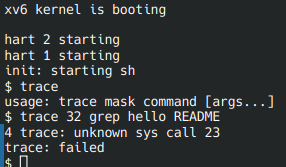
\includegraphics[width=0.72\linewidth]{part1.png}
\caption{User utility validation and syscall 23 before kernel dispatch was added}
\end{figure}

The message ``unknown sys call 23'' confirms that the user stub reached the kernel with the intended number. At this stage, the kernel has no handler registered for it.

\chapter{Kernel tracing}

\section{Mask storage and dispatch}

Each process stores its mask in \texttt{struct proc}. The \texttt{sys\_trace} handler reads argument 0 and saves it for the current process. The syscall dispatch table maps number 23 to that handler. A syscall-name table maps syscall numbers to printable names.

After dispatch returns, the kernel checks bit \texttt{num} of the process mask. When set, it prints the PID, syscall name and return value. In \texttt{fork()}, the parent's mask is copied to the child with \texttt{np->trace\_mask = p->trace\_mask}; this allows traced commands that create children to remain traced.

\section{Read-only trace}

Mask 32 has bit 5 enabled, corresponding to \texttt{SYS\_read}. Running \texttt{trace 32 grep hello README} produced:

\begin{lstlisting}
3: syscall read -> 1023
3: syscall read -> 965
3: syscall read -> 453
3: syscall read -> 0
\end{lstlisting}

The three positive results total 2441 bytes, the size of the xv6 \texttt{README}; the final zero marks end-of-file. The PID can vary between boots. The output is consistent with the screenshot and handout check.

\begin{figure}[H]
\centering
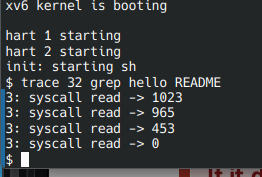
\includegraphics[width=0.72\linewidth]{part2.png}
\caption{The trace utility logging the selected read calls from grep}
\end{figure}

\chapter{Mask experiments}

\begin{enumerate}
\item With mask 32, only \texttt{read} is printed because bit 5 is set. Although \texttt{grep} opens and closes \texttt{README}, \texttt{open} is syscall 15 and \texttt{close} is syscall 21, whose bits are not selected.
\item In \texttt{trace\_mask = p->trace\_mask} inside \texttt{fork()}, each child receives its parent's mask. Therefore fork descendants also log selected calls.
\item \texttt{echo hi} writes twice: one write for \texttt{hi}, then another for the newline. The kernel prints the trace line after the first write returns, so it appears between the text and newline.
\item To select only \texttt{open} (15) and \texttt{close} (21), use \texttt{(1 << 15) | (1 << 21) = 2,129,920}.
\end{enumerate}

\utmconclusions

The syscall path is complete from the user command to kernel dispatch and reporting. Per-process mask state allows selective logging, while copying it during \texttt{fork} extends tracing to child processes. The observed mask-32 run reports exactly the selected reads, including the zero-byte end-of-file result.
\end{document}
